\documentclass[journal]{IEEEtran}
\usepackage[english]{babel}

\usepackage{amssymb, amsmath} %Paquetes matemáticos de la American Mathematical 
\usepackage[utf8]{inputenc}
\usepackage{graphicx}
\usepackage{float}
\usepackage{hyperref}
\usepackage{listings}
\usepackage{xcolor}

\definecolor{codegreen}{rgb}{0,0.6,0}
\definecolor{codegray}{rgb}{0.5,0.5,0.5}
\definecolor{codepurple}{rgb}{0.58,0,0.82}
\definecolor{backcolour}{rgb}{0.95,0.95,0.92}
% Definicio de estilo para el codigo fuente que se cita
\lstdefinestyle{mystyle}{
    backgroundcolor=\color{backcolour},   
    commentstyle=\color{codegreen},
    keywordstyle=\color{magenta},
    numberstyle=\tiny\color{codegray},
    stringstyle=\color{codepurple},
    basicstyle=\ttfamily\footnotesize,
    breakatwhitespace=false,         
    breaklines=true,                 
    captionpos=b,                    
    keepspaces=true,
    numbers=left,                    
    numbersep=5pt,                  
    showspaces=false,                
    showstringspaces=false,
    showtabs=false,                  
    tabsize=2,
}
\lstset{style=mystyle}

\renewcommand{\lstlistingname}{Código}

\ifCLASSINFOpdf

\else

\fi

\hyphenation{op-tical net-works semi-conduc-tor}


\begin{document}

\title{Ejercicio 1 - tema 5 \\ Administración de procesos}
%
\author{Vicente Romero Andrade}

\markboth{Ejercicio 1 - tema 5 Administración de procesos, Julio~2021}%
{Shell \MakeLowercase{\textit{et al.}}: }
% The only time the second header will appear is for the odd numbered pages

\maketitle


\IEEEpeerreviewmaketitle

\section{Objetivo}
% The very first letter is a 2 line initial drop letter followed

\IEEEPARstart{E}{l} objetivo es comprender y practicar el uso del modo dedicado y  
compartido empleado para crear conexiones hacia una instancia de base de datos.    
Revisar y familiarizarse con el uso de las vistas del diccionario de datos asociadas con sesiones, 
procesos de background y procesos foreground.

\section{Desarrollo}
\subsection{C1.  Código empleado para crear y poblar la tabla t01\_sga\_components}
\begin{lstlisting}[language=sql, caption=t01\_sga\_components,label={lst:codigo1}]
declare
  v_count number;
  v_username varchar2(30) := 'VRA0401';
begin
  select count(*) into v_count
  from all_tables
  where table_name='T01_SGA_COMPONENTS'
  and owner = v_username;
  if v_count > 0 then
    execute immediate 'drop table '|| v_username ||'.'||'t01_sga_components';
  end if;
  execute immediate 'create table '|| v_username ||'.'||'t01_sga_components(
    memory_target_param number,
    fixed_size number,
    variable_size number, 
    database_buffers number, 
    redo_buffers number,
    total_sga number
    )';
end;
/
insert into vra0401.t01_sga_components(
  memory_target_param_mb,
  fixed_size_mb, 
  variable_size_mb, 
  database_buffers_mb, 
  redo_buffers_mb,
  total_sg_mba
  ) 
  values (
    (select trunc(value/1048576,2) from v$parameter where name='memory_target'),
    (select trunc(value/1048576,2) from v$sga where name = 'Fixed Size'),
    (select trunc(value/1048576,2) from v$sga where name = 'Variable Size'),
    (select trunc(value/1048576,2) from v$sga where name = 'Database Buffers'),
    (select trunc(value/1048576,2) from v$sga where name = 'Redo Buffers'),
    (select SUM(trunc(value/1048576,2)) from v$sga)
  );
\end{lstlisting}
\subsection{C2. Respuesta del inciso E del punto 1.2}
\begin{figure}[H]
  \centering
  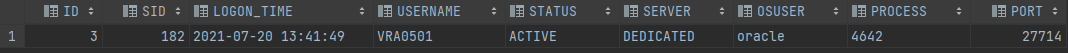
\includegraphics[scale=.50]{captura_1.png}
   \caption{catura}
   \label{fig:validador_1}
\end{figure}
\subsection{C3. Descripción de los ajustes de memoria}
\begin{figure}[H]
  \centering
  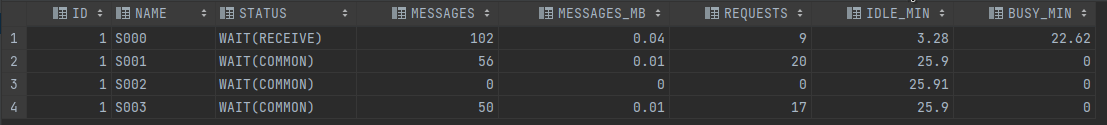
\includegraphics[scale=.40]{captura_4.png}
   \caption{tiempo de conteo}
   \label{fig:validador_2}
\end{figure}
No existio reajuste ya que existia un valor de db buffer cache adecuado para la operación a realizar.
\subsection{C4. Mostrar el contenido de cada una de las tablas t0* creadas en este ejercicio excepto la tabla de cadenas aleatorias}
\begin{figure}[H]
  \centering
  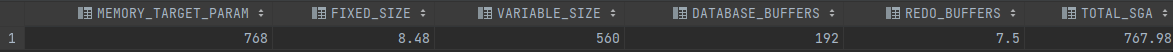
\includegraphics[scale=.20]{captura_t01.png}
   \caption{tabla t01}
   \label{fig:validador_t01}
\end{figure}
\begin{figure}[H]
  \centering
  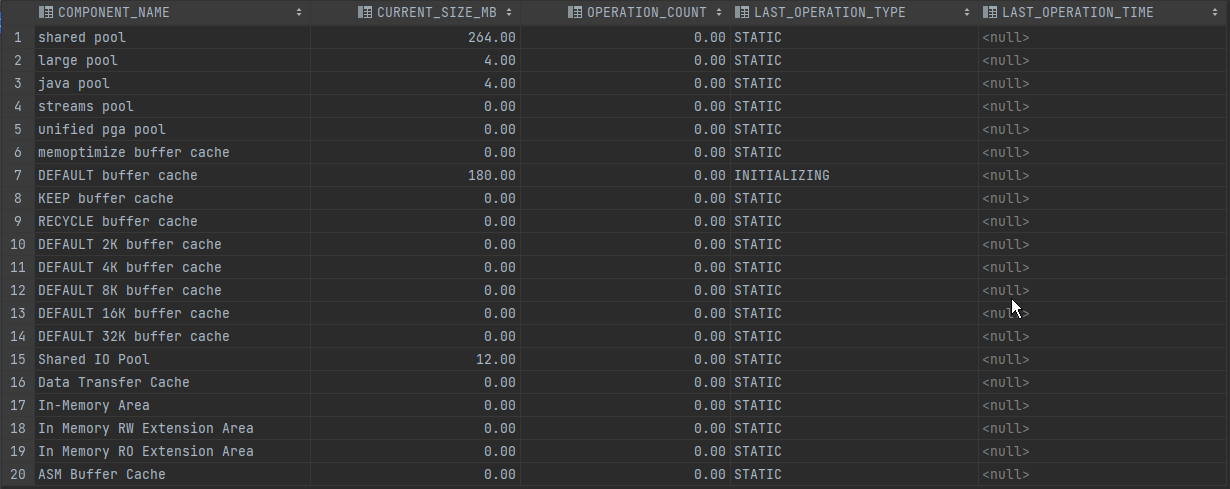
\includegraphics[scale=.20]{captura_t02.png}
   \caption{tabla t02}
   \label{fig:validador_t02}
\end{figure}
\begin{figure}[H]
  \centering
  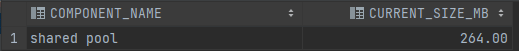
\includegraphics[scale=.40]{captura_t03.png}
   \caption{tabla t03}
   \label{fig:validador_t03}
\end{figure}
\begin{figure}[H]
  \centering
  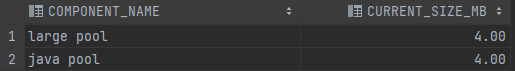
\includegraphics[scale=.40]{captura_t04.png}
   \caption{tabla t04}
   \label{fig:validador_t04}
\end{figure}
\begin{figure}[H]
  \centering
  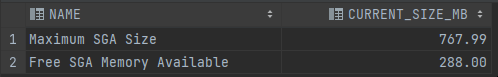
\includegraphics[scale=.40]{captura_t05.png}
   \caption{tabla t05}
   \label{fig:validador_t05}
\end{figure}
\begin{figure}[H]
  \centering
  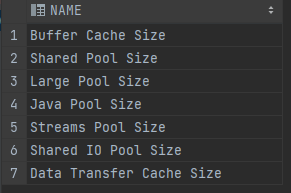
\includegraphics[scale=.40]{captura_t06.png}
   \caption{tabla t06}
   \label{fig:validador_t06}
\end{figure}
\begin{figure}[H]
  \centering
  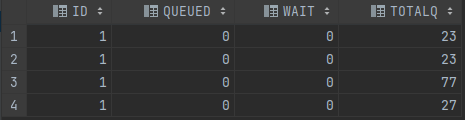
\includegraphics[scale=.20]{captura_5.png}
   \caption{tabla t07}
   \label{fig:validador_t07}
\end{figure}
\begin{figure}[H]
  \centering
  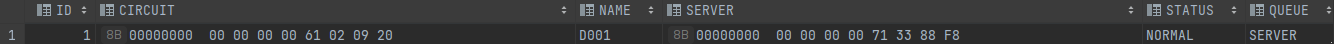
\includegraphics[scale=.20]{captura_6.png}
   \caption{tabla t07}
   \label{fig:validador_t09}
\end{figure}
\subsection{C5. Resultado del validador}
\begin{figure}[H]
  \centering
  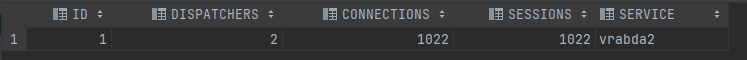
\includegraphics[scale=.20]{captura_2.png}
   \caption{resultado validador}
   \label{fig:validador_val}
\end{figure}
\section{Conclusiones}
En este ejercicio se revisaron las estructuras de memoria dentro de las areas de SGA,
fue interesante ver cuales son las que se pueden consultar usando diccionario de datos,
el unico detalle es que no se pudo apreciar la reasignación de memoria.
\ifCLASSOPTIONcaptionsoff
  \newpage

\fi

\end{document}
